\documentclass[aspectratio=169,10pt]{beamer}
\usepackage[T1]{fontenc}
\usepackage[utf8]{inputenc}
\usepackage{lmodern}
\usepackage{graphicx}
\usepackage{tikz}
\usepackage{amsmath,amssymb,booktabs,array}
\usepackage{xcolor}
\usetikzlibrary{arrows.meta,positioning,calc}
\definecolor{tecblue}{HTML}{245F80}
\definecolor{tecdeep}{HTML}{174762}
\definecolor{teclight}{HTML}{EAF2F8}
\definecolor{tecgray}{HTML}{566572}
\setbeamercolor{normal text}{fg=tecdeep,bg=white}
\setbeamercolor{frametitle}{fg=tecdeep,bg=white}
\setbeamercolor{structure}{fg=tecblue}
\setbeamercolor{block title}{fg=white,bg=tecblue}
\setbeamercolor{block body}{fg=tecdeep,bg=teclight}
\setbeamertemplate{navigation symbols}{}
\setbeamertemplate{frametitle}{\vspace{0.30cm}\hspace{0.42cm}\insertframetitle\par\vspace{0.08cm}\hspace{0.42cm}{\color{tecblue}\rule{0.88\paperwidth}{0.6pt}}}
\setbeamersize{text margin left=0.58cm,text margin right=0.58cm}
\setbeamertemplate{footline}{%
\begin{tikzpicture}[remember picture,overlay]
\node[anchor=south west,inner sep=0pt,text=tecblue,font=\scriptsize] at ([xshift=1.5cm,yshift=0.26cm]current page.south west) {OGS Training \textbar{} Dr. Eric Simo};
\node[anchor=south east,inner sep=0pt] at ([xshift=-0.36cm,yshift=0.14cm]current page.south east) {\includegraphics[height=0.88cm]{assets/bge_tec_logo.png}};
\node[anchor=south east,inner sep=0pt,text=tecgray,font=\tiny] at ([xshift=-2.25cm,yshift=0.18cm]current page.south east) {\insertframenumber};
\end{tikzpicture}\vspace{1cm}}
\newcommand{\smallnote}[1]{{\scriptsize\color{tecgray}#1}}
\newcommand{\pill}[1]{\colorbox{teclight}{\strut\hspace{0.08cm}\textcolor{tecblue}{\textbf{#1}}\hspace{0.08cm}}}
\title{Working with OpenGeoSys}
\subtitle{From geometry to verified simulation\\A 2D excavation and hydraulic-potential example}
\author{Dr. Eric Simo \textbar{} BGE TECHNOLOGY GmbH}
\date{NUMO Workshop \textbar{} 26 November 2026}
\begin{document}
\begin{frame}[plain]
\vspace{1.05cm}
{\Huge\bfseries\color{tecdeep}Working with OpenGeoSys}\par\vspace{0.32cm}
{\Large\color{tecblue}From geometry to verified simulation}\par\vspace{0.30cm}
{\large A two-dimensional excavation benchmark}\par\vspace{0.75cm}
{\color{tecgray}Dr. Eric Simo \quad | \quad BGE TECHNOLOGY GmbH}\par\vspace{0.12cm}
{\color{tecgray}NUMO Workshop \quad | \quad 26 November 2026}\par
\end{frame}
\begin{frame}{Why this example?}
\small
\begin{columns}[T,onlytextwidth]
\begin{column}{0.52\textwidth}
\vspace{0.15cm}
\begin{itemize}
\item A simple physical problem with a \textbf{non-trivial geometry}
\item A clear link between model assumptions, numerical input and results
\item A complete workflow participants can inspect in Jupyter
\item Explicit \textbf{verification}: boundary values and conservation
\end{itemize}
\begin{block}{What this is}\small A compact \textbf{steady-state diffusion / potential} example. It demonstrates OGS workflows; it is not a calibrated site-specific groundwater model.\end{block}
\end{column}
\begin{column}{0.46\textwidth}\centering\includegraphics[width=\linewidth]{assets/geometry.png}\par\smallnote{Domain schematic from \texttt{excavation.geo}.}\end{column}
\end{columns}
\end{frame}
\begin{frame}{The journey: nine notebooks, one simulation}
\begin{center}
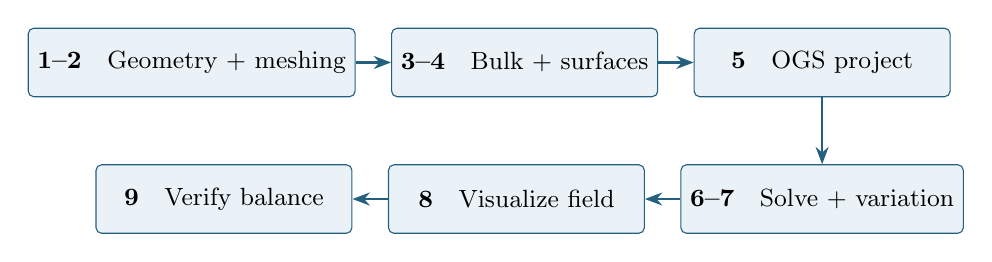
\begin{tikzpicture}[node distance=0.27cm,every node/.style={font=\small},box/.style={rounded corners=2pt,draw=tecblue,fill=teclight,minimum width=3.25cm,minimum height=0.87cm,align=center},arr/.style={-{Stealth[length=2.2mm]},thick,draw=tecblue}]
\node[box] (a) {\textbf{1--2}\quad Geometry + meshing};
\node[box,right=0.45cm of a] (b) {\textbf{3--4}\quad Bulk + surfaces};
\node[box,right=0.45cm of b] (c) {\textbf{5}\quad OGS project};
\node[box,below=0.85cm of c] (d) {\textbf{6--7}\quad Solve + variation};
\node[box,left=0.45cm of d] (e) {\textbf{8}\quad Visualize field};
\node[box,left=0.45cm of e] (f) {\textbf{9}\quad Verify balance};
\draw[arr] (a)--(b);\draw[arr] (b)--(c);\draw[arr] (c)--(d);\draw[arr] (d)--(e);\draw[arr] (e)--(f);
\end{tikzpicture}
\end{center}
\vspace{0.25cm}
\begin{block}{Today's format}\small First: understand the physical and numerical steps. Next: open the corresponding Jupyter notebooks and inspect the actual inputs, calculations and figures.\end{block}
\end{frame}
\begin{frame}{Step 1 \quad Define the geometry}
\begin{columns}[T,onlytextwidth]
\begin{column}{0.59\textwidth}\centering\includegraphics[width=\linewidth]{assets/geometry.png}\end{column}
\begin{column}{0.40\textwidth}
\begin{itemize}
\item Rectangle: \textbf{65 m} wide and \textbf{30 m} high
\item Vertical wall/notch centered at $x=32.5$ m
\item Wall thickness: \textbf{0.2 m}
\item Wall toe: $y=8$ m
\item The white slit is \textbf{excluded material}, not a separate material region
\end{itemize}
\end{column}
\end{columns}
\vspace{0.15cm}\smallnote{Source: \texttt{geometry/excavation.geo}; Step 1: \texttt{01\_geometry.ipynb}.}
\end{frame}
\begin{frame}{Step 2 \quad Turn the geometry into a mesh}
\begin{columns}[T,onlytextwidth]
\begin{column}{0.61\textwidth}\centering\includegraphics[width=\linewidth]{assets/mesh_illustrative.png}\\[-1mm]\smallnote{Illustrative triangulation, not the exact stored Gmsh mesh.}\end{column}
\begin{column}{0.38\textwidth}
\begin{itemize}
\item \textbf{Gmsh}: create 2D triangles
\item Ensure the domain is connected \textbf{below} the wall toe
\item Convert \texttt{.msh} to OGS \texttt{.vtu} via \texttt{GMSH2OGS}
\item Check geometry, topology and material IDs
\end{itemize}
\end{column}
\end{columns}
\vspace{0.2cm}\begin{block}{Essential idea}\small The bulk is \textbf{one material region (MaterialID = 0)}. The wall is represented as a geometric void with impermeable faces.\end{block}
\end{frame}
\begin{frame}{Steps 3--4 \quad Identify materials and boundaries}
\small
\begin{columns}[T,onlytextwidth]
\begin{column}{0.57\textwidth}\centering\includegraphics[width=\linewidth]{assets/geometry.png}\end{column}
\begin{column}{0.42\textwidth}
\vspace{0.1cm}
\pill{Bulk mesh}\quad \texttt{excavation.vtu}\\[0.25cm]
\pill{Left top}\quad \texttt{excavation\_101.vtu}\\[0.25cm]
\pill{Right top}\quad \texttt{excavation\_102.vtu}\\[0.26cm]
\begin{itemize}
\item Assign distinct boundary submeshes to the two top sections
\item Wall faces, bottom and external sides carry natural zero-flux conditions
\item Validate which faces receive the Dirichlet data
\end{itemize}
\end{column}
\end{columns}
\end{frame}
\begin{frame}{Step 5 \quad Specify the mathematical problem}
\small
\begin{columns}[T,onlytextwidth]
\begin{column}{0.50\textwidth}
\begin{block}{Steady-state diffusion}\vspace{-0.1cm}\[\nabla\!\cdot\!\bigl(D\nabla u\bigr)=0,\qquad D=1.\]\vspace{-0.2cm}\end{block}
\begin{block}{Boundary conditions}\vspace{-0.14cm}\[u=60\text{ (top left)},\quad u=30\text{ (top right)}\]\vspace{-0.18cm}\[\mathbf n\cdot D\nabla u=0\text{ on remaining boundaries.}\]\vspace{-0.15cm}\end{block}
\end{column}
\begin{column}{0.47\textwidth}
\begin{itemize}
\item OGS process: \texttt{SteadyStateDiffusion}
\item Scalar output array named \texttt{pressure}; physically interpreted here as \textbf{model potential}
\item Initial value $u_0=45$; single time step to the steady solution
\item No physical units inferred for $u$, $D$ or integrated reactions
\end{itemize}
\end{column}
\end{columns}
\vspace{0.15cm}\smallnote{Source: \texttt{models/excavation.prj} and \texttt{models/SteadyStateDiffusion.xml}.}
\end{frame}
\begin{frame}{Steps 5--6 \quad From OGS configuration to solution}
\begin{columns}[T,onlytextwidth]
\begin{column}{0.47\textwidth}
\begin{block}{OGS project file}\small
\texttt{excavation.prj} defines:
\begin{itemize}\item bulk and boundary meshes
\item process and medium properties
\item initial and boundary parameters
\item solver settings and output fields\end{itemize}
\end{block}
\end{column}
\begin{column}{0.50\textwidth}
\begin{block}{Run and output}\small
\texttt{ogs -o results models/excavation.prj}\\[0.2cm]
Generated \texttt{.vtu} results contain:
\begin{itemize}\item \texttt{pressure}: nodal potential\item \texttt{v}: flux vector\end{itemize}
\end{block}
\end{column}
\end{columns}
\vspace{0.2cm}
\begin{center}\Large\color{tecblue}Input geometry $\longrightarrow$ mesh $\longrightarrow$ FEM solution $\longrightarrow$ VTU\end{center}
\end{frame}
\begin{frame}{Step 7 \quad Change one boundary condition}
\begin{columns}[T,onlytextwidth]
\begin{column}{0.53\textwidth}
\begin{tabular}{lcc}\toprule
 & Reference & Exercise\\\midrule
Top-left potential & 60 & 50\\
Top-right potential & 30 & 30\\
Potential difference & 30 & 20\\
Diffusion coefficient & 1 & 1\\\bottomrule
\end{tabular}
\vspace{0.36cm}
\begin{block}{Question}\small What changes in the potential field and in the net flow around the wall toe?\end{block}
\end{column}
\begin{column}{0.45\textwidth}
\begin{center}\vspace{0.22cm}
{\Huge\color{tecblue}$\dfrac{20}{30}=\dfrac{2}{3}$}\\[0.35cm]
\small In this linear problem, the reaction magnitude scales with the applied potential difference.
\end{center}
\end{column}
\end{columns}
\end{frame}
\begin{frame}{Step 8 \quad Interpret the OGS result}
\small
\begin{columns}[T,onlytextwidth]
\begin{column}{0.56\textwidth}
\begin{itemize}
\item \textbf{Filled contours}: scalar potential \texttt{pressure}
\item \textbf{Equipotential lines}: constant values of the scalar field
\item \textbf{Streamlines}: directions of the exported flux vector \texttt{v}
\item Flow diverts \textbf{around the impermeable wall toe}
\item Compare reference and exercise on a \textbf{common color scale}
\end{itemize}
\end{column}
\begin{column}{0.43\textwidth}
\centering\includegraphics[width=\linewidth]{assets/geometry.png}\\
\smallnote{Geometry shown for orientation. Real simulated fields are viewed in Notebook 08.}
\end{column}
\end{columns}
\vspace{-0.14cm}\begin{block}{Interpretation warning}\footnotesize The variable name \texttt{pressure} does not by itself establish pressure units (e.g., kPa), and the \texttt{v} field must not be labeled m/s without a physical parameterisation.\end{block}
\end{frame}
\begin{frame}{Computed OGS fields: reference and exercise}
\begin{columns}[T,onlytextwidth]
\begin{column}{0.495\textwidth}
\centering\textbf{Reference: $u_L=60$, $u_R=30$}\\[0.10cm]
\includegraphics[width=\linewidth]{assets/reference_flow.png}
\end{column}
\begin{column}{0.495\textwidth}
\centering\textbf{Exercise: $u_L=50$, $u_R=30$}\\[0.10cm]
\includegraphics[width=\linewidth]{assets/exercise_flow.png}
\end{column}
\end{columns}
\vspace{0.2cm}
\begin{block}{How to read the figures}\footnotesize Colors represent the model potential (common range 30--60). Thin curves show equipotentials; blue curves follow the simulated flux field. The wall prevents flow across the slot, forcing it around the toe.\end{block}
\end{frame}
\begin{frame}{Step 9 \quad Verify conservation, not only appearance}
\small
\begin{columns}[T,onlytextwidth]
\begin{column}{0.59\textwidth}\includegraphics[width=\linewidth]{assets/flux_balance.png}\end{column}
\begin{column}{0.39\textwidth}
\begin{itemize}
\item Boundary reactions are \textbf{equal and opposite}
\item Reference: $\pm10.0450$ (model units)
\item Exercise: $\pm6.6967$ (model units)
\item Relative global imbalance: $<1.4\times10^{-13}$
\item Ratio $6.6967 / 10.0450 \approx 2/3$
\end{itemize}
\end{column}
\end{columns}
\smallnote{Values taken from stored \texttt{results/discrete\_flux\_balance.csv}; discrete FEM reactions, not physical volumetric flow rates.}
\end{frame}
\begin{frame}{What constitutes a credible numerical result?}
\begin{columns}[T,onlytextwidth]
\begin{column}{0.50\textwidth}
\begin{block}{Model definition}\begin{itemize}\item Defined geometry and boundaries\item Consistent mesh and material IDs\item Documented properties and solver\end{itemize}\end{block}
\end{column}
\begin{column}{0.48\textwidth}
\begin{block}{Verification evidence}\begin{itemize}\item Correct imposed boundary values\item Small free-DOF residual\item Discrete conservation\item Expected linear scaling\end{itemize}\end{block}
\end{column}
\end{columns}
\vspace{0.3cm}
\begin{center}\Large\bfseries\color{tecblue}A plausible plot is not yet a verified simulation.\end{center}
\end{frame}
\begin{frame}{Now: let's open Jupyter}
\begin{columns}[T,onlytextwidth]
\begin{column}{0.55\textwidth}
\begin{block}{Live workflow}\small\begin{enumerate}\item Select the working Jupyter/Python kernel\item Run \texttt{00\_environment\_check.ipynb}\item Explore steps \textbf{01--09} sequentially\item Compare $60/30$ and $50/30$ cases\item Inspect the conservation checks\end{enumerate}\end{block}
\end{column}
\begin{column}{0.43\textwidth}
\vspace{0.22cm}
\pill{Source files}\\[0.35cm]
\texttt{github.com/kuateric/ogs-workshop}\\[0.22cm]
\small \texttt{training/ogs-excavation-60min/}\\[0.46cm]
\color{tecblue}\large\bfseries Geometry $\to$ model $\to$ solution $\to$ verification
\end{column}
\end{columns}
\end{frame}
\end{document}
